\section{Comparison between CMA-ES and CE}

\subsection{Global comparison settings}
In all papers used for reference we haven't seen any experiments with different population
and parent sizes presented side-by-side. All the experiments we've seen
that has applied Cross Entropy to Tetris fix the population size to 100. 
However, in our upcoming experiments
CMA and CE are configured with different population and parnet numbers, which means
that we cannot compare the learning curves based on iterations/generations. Instead as described
in section \ref{varifyofce}, using the  
\textit{number of games played} as comparison reference, equal terms are secured for both algorithms 
in regards to learning speed. \\
Hence x-axis shows the total number 
of Tetris games evaluated, 
$\sum_{i = 1}^{\generation} \populationSize \numberOfEvaluations$. 
Meanwhile the y-axis still represents the mean score 
of the centroid agent at iteration $\generation$.

\subsection{Initial comparison - Bertsekas}
For the initial comparison we use the Bertsekas featureset, since the same featureset
was used for verifying the Cross Entropy implementation. Furthermore, others researchers
has used the Bertsekas featureset as a benchmarking standpoint \citep{thiery:09} \&
\citep{szita:06}.\\
The goal of this comparison is to get an initial idea of how the Shark implementation of
CMA compares to Cross Entropy.\\

\textbf{Results}

\comment{- More statistical results, multilevel model, etc.}\\

Using Cross Entropy with the constant noise setting and CMA with an initial step-size
of $0.5$, we get the following results, seen in figure \ref{fig:CMA_VS_CE_00}.\\

\begin{figure}[H]
\begin{tikzpicture}
\cmaCePlot
\end{tikzpicture}
\caption{Initial comparison between CMA-ES and Cross Entropy \label{fig:CMA_VS_CE_00}}
\end{figure}

As figure \ref{fig:CMA_VS_CE_00} reveals that CMA converges faster,
but reaches a local optimum at around 2,000 games played. Meanwhile CE has a 
slower convergence but reaches a better mean score compared to CM at around 5,500
agents evaluated. In detail, CMA on average reaches a score of 50,000 rows, and
CE reaches a score of 100,000.\\

\textbf{Analysis and discussion}

These results clearly defy our initial hypothesis as we predicted
for CMA to outperform CE, due to its more sophisticated nature. 
One reason for this outcome could possibly be that
CMA has a very little population size compared to Cross Entropy,
which could be a decisive lack as the objective function is noisy with 
a high variance. These results indicate a need to adjust the CMA
configuration, to prevent the too fast convergance.

Among the possible adjustments are:\\
\\
\textit{Enlargment of population size}\\
As the population size is quite small (only around 13)
for this experiment, the CMA algorithm might not be able
extract enough information at each generation. As seen in 
section \ref{optimalsettingsce}, CE looses performance as 
thepopulation size is set too low. This might be a problem 
that counts for CMA as well. In figure \ref{fig:CMA_VS_CE_00},
the CMA algorithm has much the same shape as \\
\\
\textit{Evaluate each agent multiple times}\\
A posible source of poor performance could be 
that the ranking of agents becomes very difficult
due to high noise. To better verify the actual
performance of an agent, it could be evaluated 
multiple times and let the mean of the evaluations
determine it's ranking.\\
\\
\textit{Change the recombination type}\\
As described in section \ref{CMAtheory}, 
the CMA algorithm is not bound to update its 
new mean to just the centroid of the selected 
vectors. Instead, it can weight better solutions
more heavily when moving its mean. When doing so,
it risks biasing vectors that appear to be better 
but in reality, just by faulty ranking, should
not be considered a good agent.\\
\\
None of the experiments seen so far has allowed a 
consistent mean score of more 
than 200,000. This brings concern into 
consideration, that it might be the objective function
that poses a natural limit on the score.
In this case the objective function
models playing Tetris with the Bertsekas featureset. 
It is unkown to us
whether it's possible to construct an agent 
with a mean score of more than
200,000 lines on average. 
Yet, as our aim is not to find the best controller,
untill both algorithms reaches the same upper limit 
of scores theres is no need
to alter the featureset just to
expand the maximum score reachable.\\
\\
Yet, to minimize the likelihood 
that the featureset were the cause of the 
poor performance of CMA, it seemed 
appropiate to conduct a similar comparison 
using another featureset. 
To speed up the process, the game difficulty were 
adujsted to casue agents to fail faster.
The increased difficulty and alternate
featureset is described in 
further detail in section \ref{compoffeatureset}.

\subsection{Comparison of featuresets  \label{compoffeatureset}}

The best configurations of the experiments using the Bertsekas
featureset never appears to score much higher than 200,000 lines
on average. Due to this, the question of whether the specific featureset
causes rapid convergence remains.\\
To address this, both CMA-ES and Cross
Entropy experiments were run 30 times with respectively the Bertsekas and 
Dellacherie featureset. To prevent long runtimes, the games were simulated
using a harder version of Tetris referred to as 'Hard Tetris'. With regular 
Tetris, all pieces occur with equal likelihood.\\
%(see figure \ref{fig:TetrisPieces})
To increase the difficulty of the game,
in our hard Tetris, the s-block and z-block appear twice as often 
as the other pieces.

\begin{figure}[H]
\begin{center}
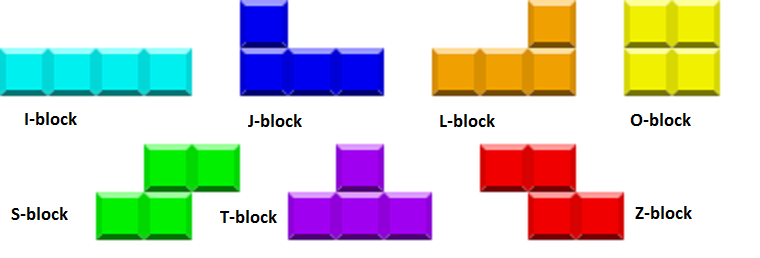
\includegraphics[scale=0.6]{img/Pieces}
\end{center}
\caption{Regular Tetris pieces \label{fig:TetrisPieces}}
\end{figure}

\textbf{Results}

In the following figures the mean results of 30 runs of both CMA and Cross 
Entropy is presented. The settings for Cross Entropy remains at constant noise
with a noise term of $z_t = 4$ and an initial sigma of $\sigma_0 = 100.$, 
and the CMA with $\sigma_0 = 1$.\\
\\
Figure \ref{fig:featuresetCompareBertsekas} shows the experiment with the 
Bertsekas featureset. This shows that when running the algorithms with a
harder game, the algorithms behave mostly the same as with regular 
Tetris. Namely that CMA converges faster than Cross Entropy, 
but is eventually outperformed.

\begin{figure}[H]
\begin{tikzpicture}
\plotBertsekasCmaVsCEHardTetris
\end{tikzpicture}
\caption{Comparison between CMA-ES and Cross Entropy 
using hard Tetris and the Bertsekas featureset 
\label{fig:featuresetCompareBertsekas}}
\end{figure}

When using the Dellacherie featureset a similar behaviour is observed.
However, the convergence seems to occur earlier and with a higher score
(figure \ref{fig:featuresetCompareDellacherie}).

\begin{figure}[H]
\begin{tikzpicture}
\plotDellCmaVsCEHardTetris
\end{tikzpicture}
\caption{Comparison between CMA-ES and Cross Entropy 
using hard Tetris and the Dellacherie featureset
\label{fig:featuresetCompareDellacherie}}
\end{figure}

\comment
{
Add full data graphs as appendix.
}



\textbf{Analysis and discussion}

The experiment with different featuresets indicates that the behaviour 
is not heavily dependant on the featureset, as the development of the 
graphs closely resemble the initial comparison experiment.
Furthermore, it appears that increasing the difficulty of the game
simple shifts the score, but does not affect the development of the graphs.
Therefore, we conclude that changing the featureset does not invalidate
the comparison of the two optimization algorithms.
\comment{
We will also consider it valid to simulate using the faster
hard Tetris when comparing CMA against Cross Entropy.
}

\subsection{Configuration of CMA}

In previous sections we focused on tuning Cross Entropy for the Tetris 
problem. Whereas we deliberately chose not to tune CMA due to its implementation 
into the Shark library \citep{shark08}. However, experiments with the "out of 
the box" CMA from Shark, with default settings vs the tuned Cross Entropy
resulted in CMA reaching convergence very fast but not achieving the same point
limit as Cross Entropy.\\
By adjusting the population size to that similar of Cross Entropy, we are able
to get a fair comparison between the two algorithms, given each generation will
contain the same number of agents. By setting the population and offspring size
to the same values, we in effect test if the covariance matrix and the step-size
control has a impact on the algorithm performance compared to Cross Entropy
which does not have the features.\\
Furthermore, CMA also has a unique formula for calculating the updated mean,
called the 'Recombination type' \ref{CMAtheory}. Where the recombination type
determines how much influence each of the offspring vectors has on the next
generation. Built into the CMA algorithm is three methods of recombination. 
\begin{itemize}
\item EQUAL, Each of the offspring vectors has equal influence in the generated mean. Each has $w_i = 1$.
\item LINEAR, The best of the offspring vectors has more influence. 
\item SUPERLINEAR, The vectors are weighted with a logarithmic equation. $w_i = \frac{w_i'}{\sum_{j=1}^{\mu} w_j'^+}$
\end{itemize}
As default, CMA uses Super Linear recombination. However, Tetris is a problem
with multiple local optimums in its solution space. This means, though a vector may be the best in its generation, it could be a nearby local optimum. Therefore, Super Linear recombination may not be the optimal recombination type for the Tetris problem.\\
\comment{Discuss games per. agent, featuresets, Tetris difficulties, total agent evaluation / stopping criteria, parent size.}
\\
\comment{Was about to list the experiment setup (population/offspring with recombination type - wait for Oswin conversation to end), will perform experiments with hard tetris}\\
\\
\comment{Reference to CMA-ES section needs to be fixed}\\
\comment{Weights for recombination could have a symbol? (change policy weight
symbol?)}\\
\comment{Find Linear combination type formula of change format of itemize list}

\textbf{Results}

%\begin{tabular}{l l | l l l }
% & \multicolumn{1}{r|}{$\populationSize / \offspringNumber$} & (22/8) & (50/10) %& (100/10)
%\multicolumn{1}{l}{Recombination type} & &  &  & \\
%\hline
%\multicolumn{2}{l|}{Equal / $w_i = \frac{1}{\sum_{j=1}^{\offspringNumber} w_j}$}}  & & &
%\end{tabular}

\textbf{Analysis and discussion}


\subsection{Dynamic games played per agent}

\comment{Indledenede tekst}

\textbf{Results}

\comment{- WHAT results did the comparison yield}\\
\comment{- Show results from comparison experiments}


\textbf{Analysis and discussion}

\comment{- WHY did we get these results}\\
\comment{- Discuss the results of the comparison experiments}
